\documentclass[10pt,a4paper]{article}
\usepackage[utf8]{inputenc}
\usepackage[T1]{fontenc}
\usepackage{lmodern}
\usepackage[margin=1.5cm, top=1.4cm, bottom=1.4cm]{geometry}
\usepackage{hyperref}
\usepackage{enumitem}
\usepackage{titlesec}
\usepackage{xcolor}
\usepackage{graphicx}

\definecolor{accent}{HTML}{00686E}
\hypersetup{colorlinks=true, urlcolor=accent, linkcolor=accent}
\pagenumbering{arabic}
\setlength{\parindent}{0pt}

\titleformat{\section}{\large\bfseries\color{accent}}{}{0em}{}[\vspace{-0.6em}\rule{\textwidth}{0.8pt}]
\titlespacing{\section}{0pt}{7pt}{4pt}

\newcommand{\role}[4]{%
  \textbf{#1} \hfill \textbf{#2}\\[1pt]%
  \textit{#3} \hfill \textit{#4}\\[2pt]%
}
\setlist[itemize]{leftmargin=1.2em, itemsep=1.5pt, topsep=2pt, parsep=0pt}

\begin{document}

% ================= HEADER =================
\begin{minipage}[c]{0.80\textwidth}
  {\Huge\bfseries Prabhavit Gupta}\\[3pt]
  {\color{accent}\large Software Systems Engineer: Python, TypeScript, Automation \& Cloud Services}\\[6pt]
  {\footnotesize +39 351 610 7807 ~$\vert$~
  \href{mailto:prabhavitg@gmail.com}{prabhavitg@gmail.com} ~$\vert$~
  \href{https://www.linkedin.com/in/prabhavit/}{linkedin.com/in/prabhavit} ~$\vert$~
  \href{https://github.com/prab-gupta}{github.com/prab-gupta} ~$\vert$~
  Venice, Italy (CET Time Zone / EU Permanent Resident)}
\end{minipage}\hfill
\begin{minipage}[c]{0.18\textwidth}
  \raggedleft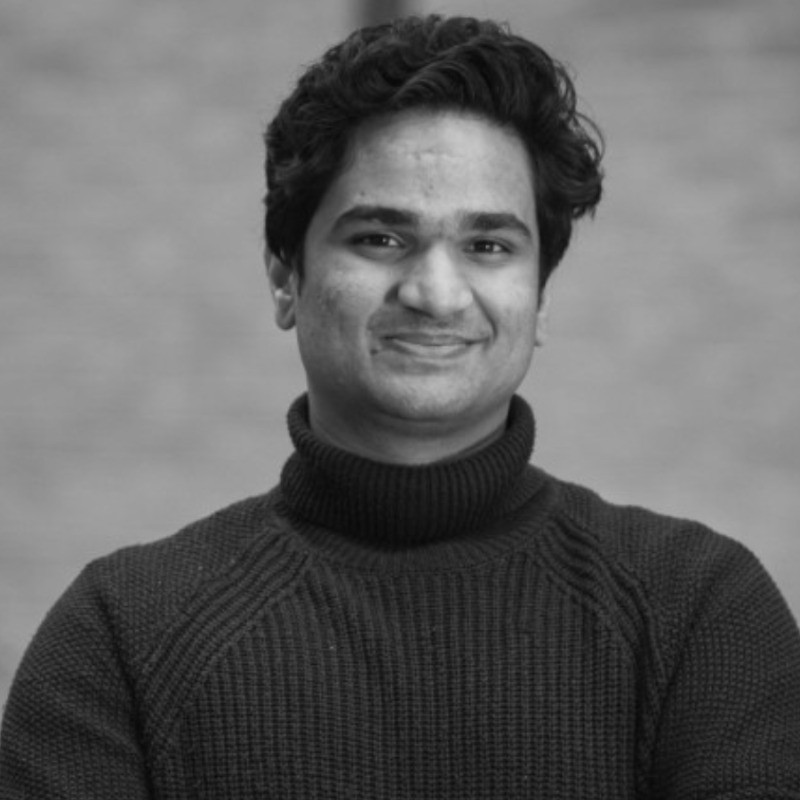
\includegraphics[width=2.0cm]{photo.jpg}
\end{minipage}
\vspace{-2pt}

% ================= SUMMARY =================
\section{Summary}
Software Systems Engineer with 3 years of commercial production experience architecting, implementing, and deploying high-availability software that integrates cloud backends with physical and operational automation pipelines. Strong background in Python, TypeScript, C++, and Linux environments, with demonstrated expertise building resilient microservices, diagnostic telemetry, and AI-assisted automation tooling. Ca' Foscari University of Venice alumnus based in Venice, Italy (CET time zone) with an EU Long-Term Residence Permit (permanent unrestricted EU work authorization); available immediately for full-time remote contract roles.

% ================= TECHNICAL EXPERTISE =================
\section{Technical Expertise}
\begin{itemize}
  \item \textbf{Software Development \& Architecture:} Python (asyncio, FastAPI, PyTorch, NumPy, Pydantic), TypeScript / JavaScript, C++, low-level network and device communication protocols, distributed microservice patterns.
  \item \textbf{Cloud Infrastructure \& DevOps:} AWS services, infrastructure-as-code automation (AWS CDK / CloudFormation), Docker containerization, CI/CD pipeline automation with GitHub Actions, Linux system internals.
  \item \textbf{Telemetry \& System Reliability:} Distributed monitoring, Prometheus/Grafana metrics, automated alerting, diagnostic logging frameworks, and root-cause debugging under high operational loads.
  \item \textbf{Applied AI \& Automation:} Tool-calling autonomous agents, Model Context Protocol (MCP), LLM-backed operational workflows, Claude Code for automated regression testing and high-velocity delivery.
  \item \textbf{Databases \& Data Stores:} PostgreSQL (schema design, indexing, transactional integrity), Redis (caching, queues, distributed locks), structured telemetry storage.
  \item \textbf{Languages \& Authorization:} English (C1 Professional, fluent), Hindi (Native), Italian (Conversational). EU Long-Term Residence Permit (unrestricted EU work authorization across all EU member states, no sponsorship required).
\end{itemize}

% ================= EXPERIENCE =================
\section{Experience}

\role{\href{https://flowspace.co}{FlowSpace.co}}{Mar 2024 - Aug 2026}{Software \& AI Automation Engineer}{London, UK (remote)}
\begin{itemize}
  \item Designed and operated scalable distributed software microservices in Python and TypeScript, supporting 4,500+ active enterprise users with 99.8\% production reliability.
  \item Integrated cloud-based backend services with operational automation workflows, building event-driven message queues and reliable error recovery mechanisms.
  \item Implemented health-check monitoring, real-time alerting, and automated diagnostic tools across Linux containerized environments to ensure continuous operational uptime.
  \item Built AI-assisted automation pipelines using Claude and custom tool-calling agents, streamlining operational workflows and eliminating repetitive administrative tasks.
  \item Maintained strict continuous integration and automated testing routines with GitHub Actions and Playwright, preventing production regressions.
\end{itemize}

\role{Urlink}{Apr 2025 - Jul 2025}{Software Solutions Developer (Freelance)}{Barcelona, Spain (remote)}
\begin{itemize}
  \item Developed backend integration modules and API connectors linking third-party cloud services with distributed database clusters.
  \item Optimized data ingestion pipelines and database queries in PostgreSQL, eliminating concurrency bottlenecks and ensuring data consistency.
  \item Engineered automated system telemetry and error logging harnesses to monitor data pipeline health and flag anomalous spikes in real time.
\end{itemize}

\role{Independent Technical Consultant}{Aug 2023 - Feb 2024}{Software \& Automation Developer}{Venice, Italy}
\begin{itemize}
  \item Built custom software tools, asynchronous data processing pipelines, and API integrations using Python and C++ for European SMB clients.
  \item Automated internal system workflows and device data reporting routines, reducing manual troubleshooting overhead for technical client teams.
  \item Authored technical architecture specifications, deployment guides, and maintenance runbooks for Linux production systems.
\end{itemize}

% ================= EDUCATION =================
\section{Education}
\role{Ca' Foscari University of Venice}{2020 - 2024}{BA in Philosophy, International Studies and Economics}{Venice, Italy}
\begin{itemize}
  \item Rigorous foundational coursework in formal mathematical logic, decision theory, analytical systems modeling, and epistemological frameworks.
\end{itemize}

\end{document}
